\documentclass[12pt]{article}
\usepackage{url}
\usepackage{graphicx}
\usepackage{float}
\usepackage{amsmath}
\usepackage{amsfonts}
\usepackage{amssymb}

\title{\bf Fortran Modernisation Workshop - \\ 
       Current Usage of Software Engineering}
\author{Wadud Miah\footnote{wadud.miah@nag.co.uk}, Filippo Spiga\footnote{fs395@cam.ac.uk}, Fatima Chami\footnote{fatima.chami@durham.ac.uk}, Kyle Fernandes\footnote{kj333@cam.ac.uk}}
\date{\today}

\begin{document}
\maketitle

\begin{abstract}
This article will present the results of the usage of software engineering
practices by the academic computational science community who use the Fortran
programming language. The statistics were gathered from running
the Fortran Modernisation Workshop. 
\end{abstract}
%
\section{Introduction}
The Fortran Modernisation Workshop~\cite{fmw:nag} has been running in the UK
and a number of workshops have been scheduled. The registration process gathers
data from the computational science community who use the Fortran programming
language and asked the following question:
\begin{enumerate}
\item Which Fortran standard are you using? Fortran 66, 77, 90, 95, 2003, 2008 and
object oriented programming (OOP);
\item Are you using any software engineering techniques for code development?
\item Are you using any unit testing frameworks for Fortran?
\item Are you using any in-situ visualisation libraries in Fortran?
\item Are you using any version control system?
\end{enumerate}
The results of the above questions are described below and their ramifications.
The Fortran Modernisation Workshop covers the following topics:
\begin{itemize}
\item Software engineering for computational science;
\item Modern Fortran standards and how to write optimized and efficient Fortran;
\item NetCDF and HDF5 scientific file formats for data sharing in Fortran;
\item GNU Automake to automate the build process;
\item pFUnit unit testing framework for testing Fortran codes;
\item Doxygen for Fortran code documentation;
\item Git version control for collaborative code development;
\item In-memory visualisation using PLplot in Fortran;
\item IEEE Floating Point Exception Handling
\item Fortran interoperability with C, Python and R;
\end{itemize}
This article will argue that there is a clear need to run the Fortran Modernisation 
Workshop. 
%
\section{Fortran Standards Usage}
The current usage of Fortran standards is shown in Figure~\ref{fortran_usage:png}
which shows there is still usage of the Fortran 77 standard which is a nearly 40 year
old standard. Fortran 90 is mostly used which is expected as it was a major revision of
the Fortran language. Usage of Fortran 2003 and 2008 is still lacking which still 
requires promoting within the community. In addition, adoption of object oriented 
programming (OOP) is still widely lacking which also needs to be promoted within the
community.  
\begin{figure}[H]
\begin{center}
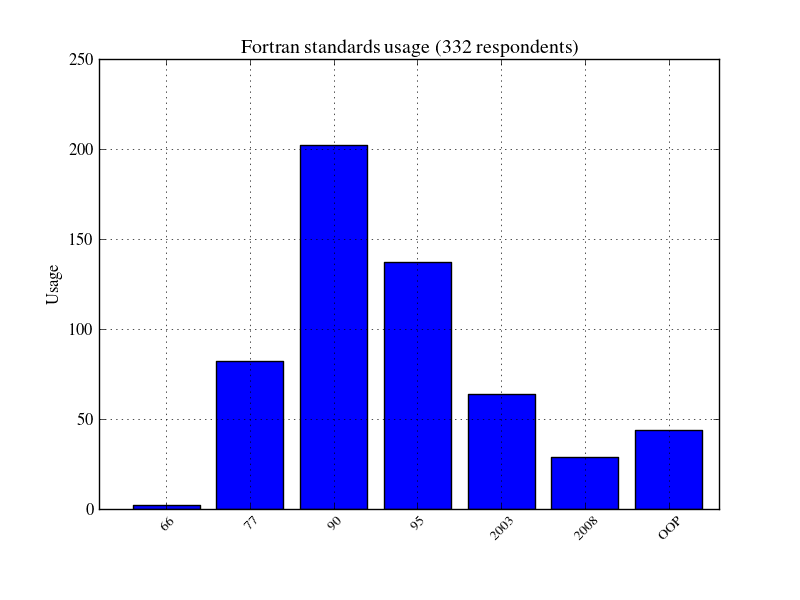
\includegraphics[width=13cm,height=9cm]{fortran_usage.png}
\caption{Fortran standards usage}\label{fortran_usage:png}
\end{center}
\end{figure}
The aim of the Fortran Modernisation Workshop is to stop people using the Fortran 77 
standard (unless they are maintaining legacy code) and increase the usage of Fortran
2003 and 2008, as well as wider use of object oriented programming. 
%
\section{Software Engineering Techniques} \label{softeng}
The usage of software engineering techniques used by the community is shown 
in Figure~\ref{softeng:png}. 
\begin{figure}[H]
\begin{center}
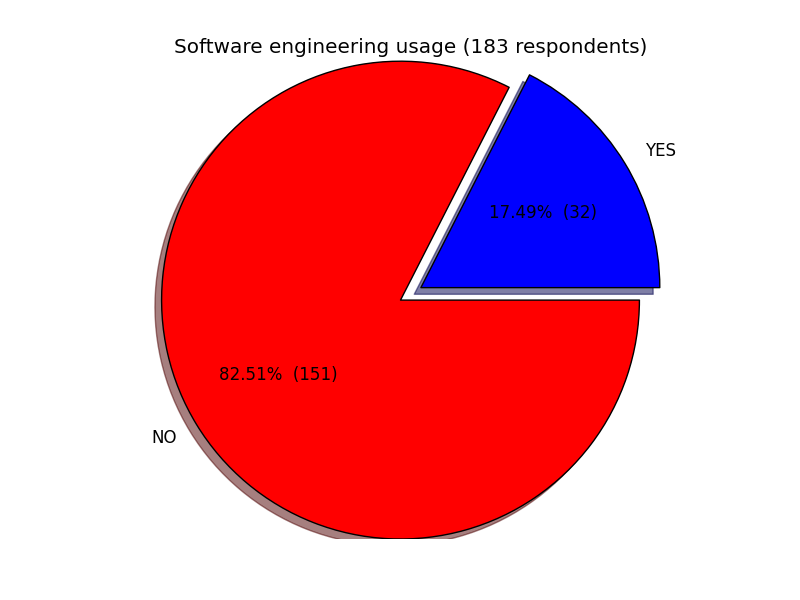
\includegraphics[width=8cm,height=6cm]{softeng.png}
\caption{Usage of software engineering techniques}\label{softeng:png}
\end{center}
\end{figure}
Figure~\ref{softeng:png} shows the vast majority of the Fortran
code development community (82\%) are not using any software engineering techniques.
%
\section{Unit Testing Frameworks}\label{utf}
The usage of unit testing frameworks used by the community is shown in
Figure~\ref{pfunit:png}
\begin{figure}[H]
\begin{center}
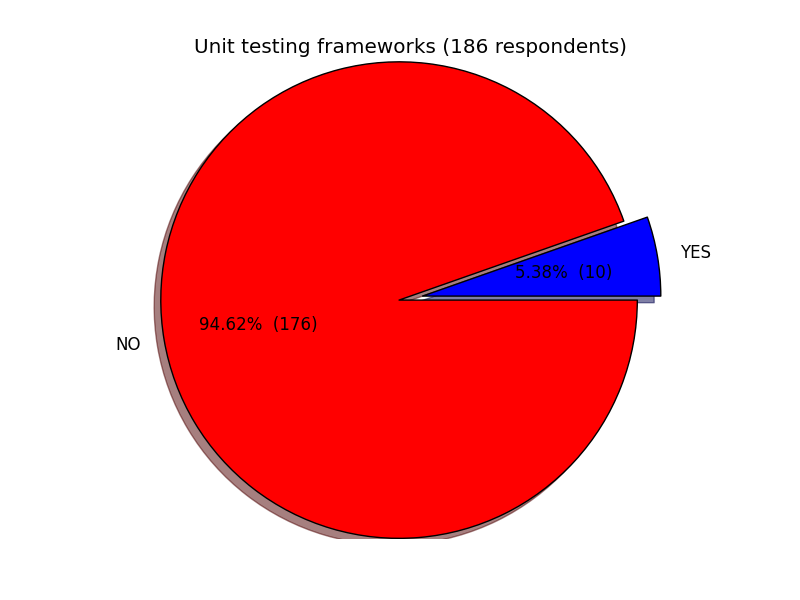
\includegraphics[width=8cm,height=6cm]{pfunit.png}
\caption{Usage of unit testing frameworks}\label{pfunit:png}
\end{center}
\end{figure}
Figure~\ref{pfunit:png} shows that 94\% of the community are not using any
unit testing frameworks. This is not to say that 94\% of the community are not
testing their codes, but unit testing frameworks do simplify the process of
testing which results in higher quality codes and better research. 
%
\section{In-situ Visualisation}\label{isv}
The usage of in-situ visualisation libraries used by the community is shown in 
Figure~\ref{plplot:png}
\begin{figure}[H]
\begin{center}
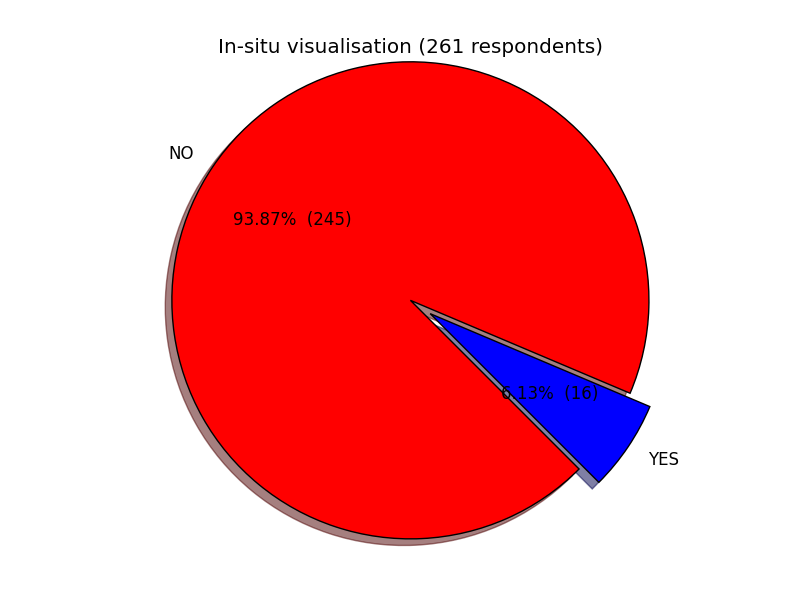
\includegraphics[width=8cm,height=6cm]{plplot.png}
\caption{Usage of in-situ visualisation libraries}\label{plplot:png}
\end{center}
\end{figure}
Figure~\ref{plplot:png} shows that 94\% of the community are not using any
in-situ visualisation techniques which means computational jobs (using LSF, PBS, SLURM) 
could be running for longer than expected. In-situ visualisation allows researchers to 
test the results of the codes whilst it is running. This is to determine whether it has 
their simulation has converged or is resulting in non-physical effects due to incorrect
models and/or parameters. If any of the described events have occurred, the computational
job can obviously be terminated, resulting in saved CPU cycles and energy, and
increased productivity for the academic researcher. 
%
\section{Version Control}\label{vc}
The usage of version control systems used by the community is shown in 
Figure~\ref{verscon:png}.
\begin{figure}[H]
\begin{center}
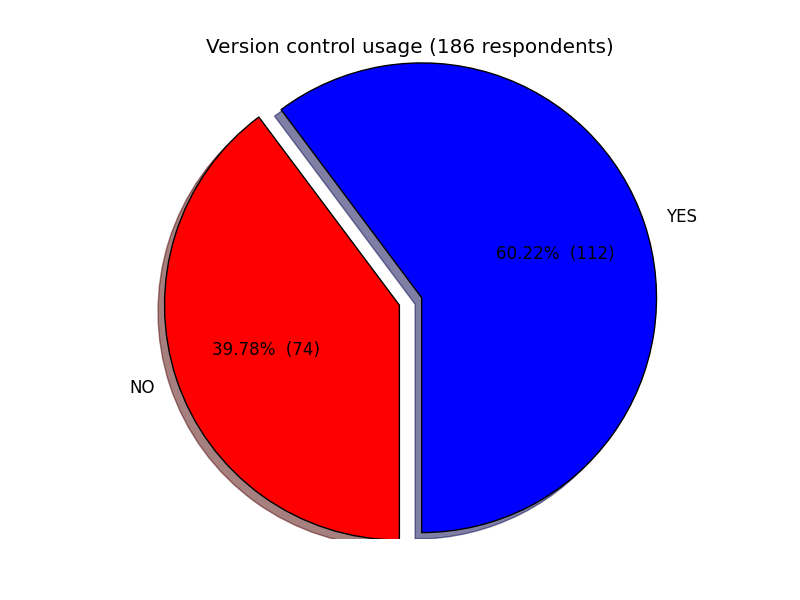
\includegraphics[width=8cm,height=6cm]{verscon.png}
\caption{Usage of version control systems}\label{verscon:png}
\end{center}
\end{figure}
Figure~\ref{verscon:png} shows 39.78\% of the community do not use version control systems
whilst 60.22\% of the community do. Version control systems are an important
tool for reproducible research as well as a tool for increased productivity, so
this needs to be addressed within the academic community. 
%
\section{Conclusion}
This article has attempted to show the need of the Fortran Modernisation Workshop
which addresses the shortfalls highlighted in the data from the registration process. 
It is the authors' view that the Fortran Modernisation Workshop will address the
shortfalls highlighted and increase the academic researcher's productivity and help them
produce better research software and better science. 
\bibliographystyle{abbrv}
\bibliography{fortran_usage}

\end{document}

